\chapter{Simulaciones numéricas}
\graphicspath{{figs/}}
\label{Simulaciones}

En este capítulo presentamos los resultados obtenidos al resolver el problema propuesto en la sección \ref{S:Modelo SIR espacial het} para los 
distintos casos de $\beta_{\vb r}$ utilizando métodos numéricos. Se utilizaron para ello técnicas de programación en paralelo para acelerar la
velocidad de cómputo. En el apéndice \ref{C:ap1} puede encontrarse la descripción de la metodología numérica utilizada, que consiste en un esquema simple de 
diferencias finitas sobre una grilla regular.

Todas las simulaciones realizadas en este capítulo corresponden al problema presentado en la subsección \ref{Problema} pero con distintas distribuciones de 
$\beta_{\vb r}$. De modo que las condiciones iniciales y de contorno son las que se indican en dicha subsección, utilizando de manera 
general $\delta x=1$, $L=1024$ y $S_0=I_0=1$.\footnote{Se recomienda mirar nuevamente la subsección \ref{Problema}.} Por otro lado, cabe mencionar que en el esquema numérico se utilizó, también de manera general, una discretización 
espacial del sistema de $1024\times1024$ sitios de igual tamaño. Los demás parámetros se especificarán según corresponda y 
si los mencionados aquí fueran distintos en alguna ocasión se hará mención de ello.

\section{Medios aleatorios}

\label{S:aleatorios}
En esta sección reproducimos y validamos los resultados obtenidos por A. Kolton y K. Laneri (2019) \cite{kolton} en su trabajo sobre frentes de 
infección rugosos en medios aleatorios, donde trabajaron con la heterogeneidad dicotómica-aleatoria descrita en la sección \ref{S:Modelo SIR espacial het}. 
Adicionalmente, se muestran los resultados correspondientes al caso homogéneo de la sección \ref{S:Modelo SIR espacial hom}. De esta manera podremos visualizar 
y entender la dinámica del problema heterogéneo comparando con el caso homogéneo del cual tenemos mayor entendimiento analítico.



\subsection{Caso homogéneo}
\label{hom}
Recordemos que el problema homogéneo, donde la tasa de transmisión $\beta_{\vb r}=\beta$ es la misma en todo el espacio, es equivalente a usar la distribución 
\ref{prop} con $p=0$. Se utilizó $\beta = 1$ y $\gamma=0.2$. Se omitirán las unidades por claridad pero es importante recordar que estos valores tienen unidades 
de $1/t$ ya que son la tasa de infección y recuperación respectivamente\footnote{De manera similar se omitirán las unidades tanto de tiempo como de longitud en 
la mayoría de las ocasiones. Si esto lo incomoda mucho 
piense que las unidades de tiempo son u$_{t}$ y las de espacio u$_{l}$, poniendo $\beta$, $\gamma$, $D_{S}$ y $D_{I}$ en estas unidades la dinámica se describe 
correctamente en dichas unidades.}. Para los coeficientes de difusión se 
utilizó $D_{S}=0$ y $D_{I}=1$, los cuales deben tener dimensión de área por unidad de tiempo. Podemos ver que $\gamma/\beta=0.2<S_0=1$, de modo que según lo visto en 
la subsección \ref{ondas} es posible la propagación de la infección a través de una solución de onda.

En la figura \ref{fig:hom_case_tevol} se muestra la evolución del frente de infección/incendio para este caso. Puede observarse que el frente es asimétrico, es decir, se 
comporta de manera distinta en la parte frontal que en la parte posterior, tal como habíamos anticipado en la subsección \ref{ondas}. Se muestra también  el campo de 
desplazamiento del frente $u(y,t)$ (\ref{campo}). Puede verse que éste es completamente plano, como es de esperar para un medio homogéneo.

\begin{figure}[h]
    \centering
    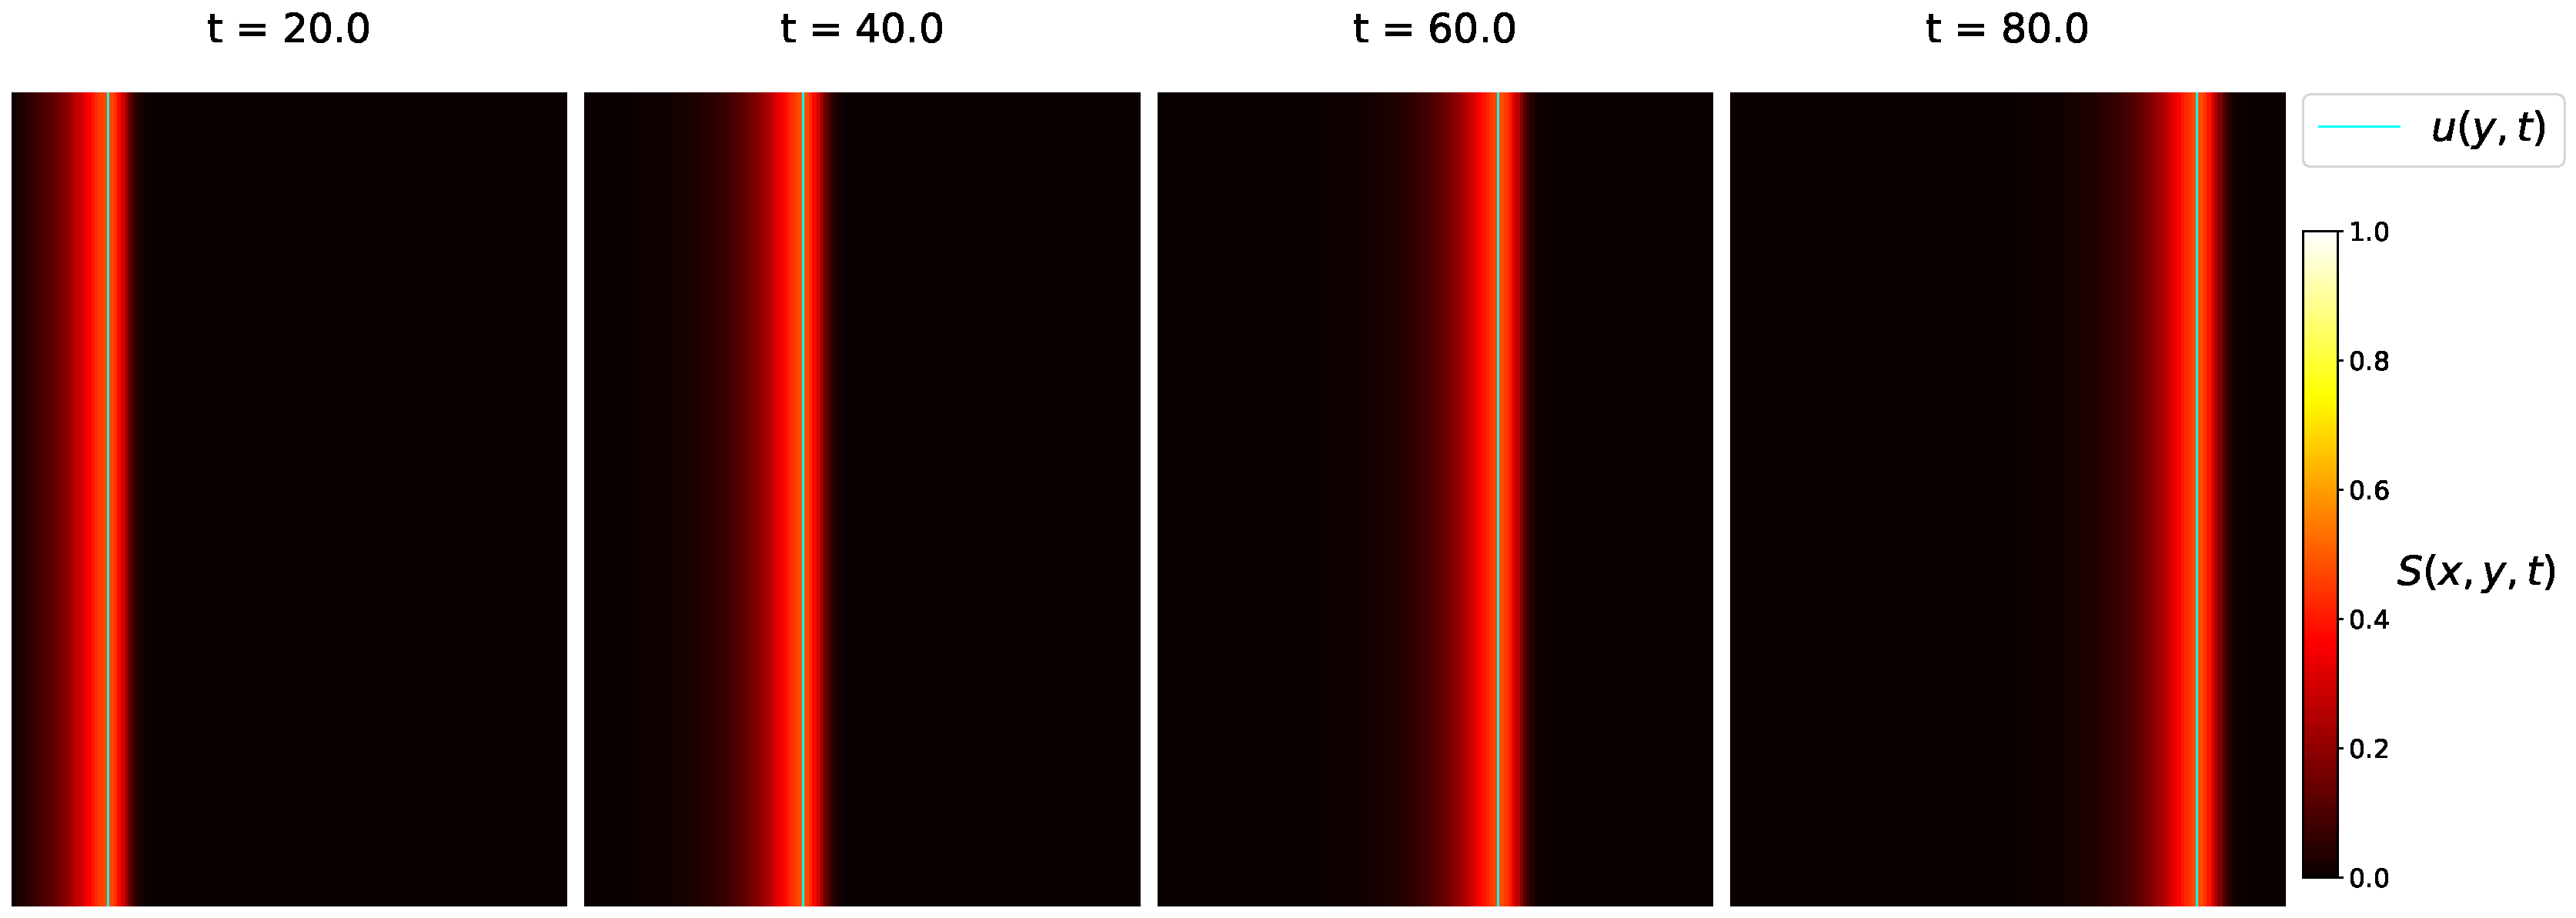
\includegraphics[width=\imsizeL]{hom_case_tevol.pdf}
    \caption{Evolución del frente de infección/incendio para el problema homogéneo.}
    \label{fig:hom_case_tevol}
\end{figure}

En la figura \ref{fig:u_cm(t)} se muestra la posición del centro de masa del frente de propagación $u_{cm}(t)$ (\ref{centromasa}) en función del tiempo para distintos valores de $\gamma/\beta$. Puede observarse 
que para el caso $\gamma/\beta=1$ el sistema cambia notablemente su comportamiento y no es posible identificar un frente de onda propagándose a velocidad constante, en 
acuerdo con la condición $\gamma/\beta<S_0=1$. Por otro lado, a partir de estos resultados se calculó la velocidad $c$ (\ref{velocidad}) para cada caso a partir de un ajuste lineal
descartando un periodo transitorio. De ello vemos que la velocidad del frente $c_0= 2\sqrt{D_I\beta(S_0-\gamma/\beta)}$ estimada en la subsección \ref{ondas} concuerda 
con las velocidades calculadas a partir de la resolución numérica con un error relativo, en promedio, de $4.5\%$. En la mayoría de los casos $c_0$ resulta 
sobreestimar levemente el valor de $c$, esto puede explicarse recordando que el valor de $c_0$ se obtuvo en una aproximación donde se supone que hay más susceptibles 
de los que realmente hay y por ello es de esperar que la velocidad $c_0$ estimada sea mayor que la real. 
\begin{figure}[h]
    \centering
    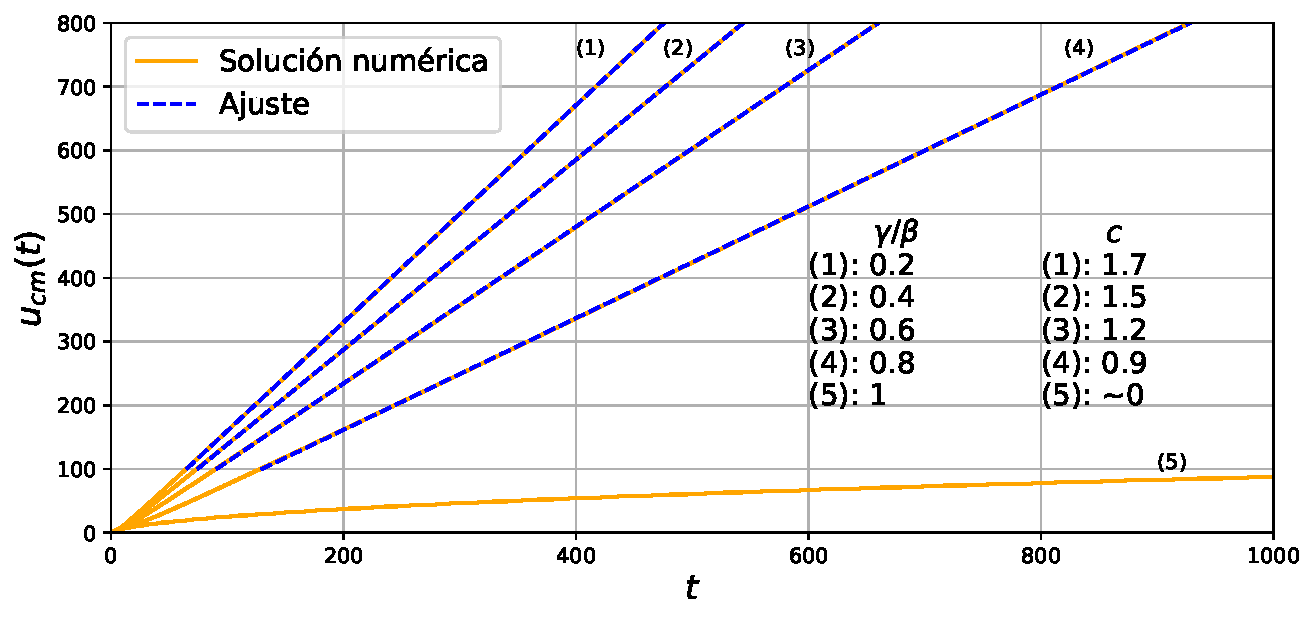
\includegraphics[width=\imsizeL]{u_cm(t).pdf}
    \caption{Posición del centro de masa del frente de propagación en función del tiempo para distintos valores de $\gamma/\beta$ junto 
    con los correspondientes ajustes lineales. Se muestra también la velocidad $c$ del frente obtenida para cada caso.}
    \label{fig:u_cm(t)}
\end{figure}

Un observable más a destacar en esta instancia es el perfil del frente de propagación $f_I(x)$ (\ref{perfil}), que se observa en la figura \ref{fig:f_I(x)} para 
$\gamma/\beta=0.2$. Se muestran también los perfiles asintóticos frontal y posterior del frente de onda calculados en la subsección \ref{ondas}, ecuaciones \ref{larika2} y 
\ref{larika} respectivamente.

\begin{figure}[h]
    \centering
    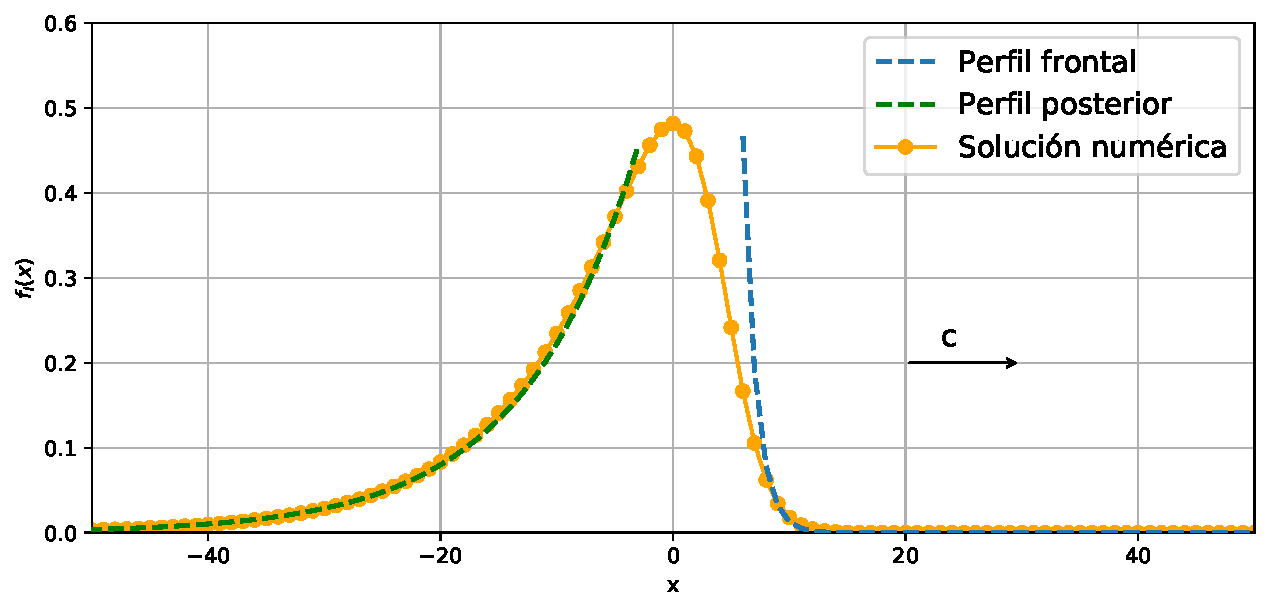
\includegraphics[width=\imsizeL]{f_I(x)_hom.pdf}
    \caption{Perfil del frente de propagación $f_I(x)$ para $\gamma/\beta=0.2$. Se muestran también los perfiles asintóticos frontal y posterior 
    del frente de onda calculados en la sección \ref{S:Modelo SIR espacial hom}.}
    \label{fig:f_I(x)}
\end{figure}

\subsection{Heterogeneidad dicotómica-aleatoria}
\label{al}

Comenzamos el estudio de la heterogeneidad dicotómica-aleatoria, con $\beta_{\vb r}$ dado por \ref{prop}, observando en la figura \ref{fig:hom_case_tevol_hetero} la
evolución temporal del frente de infección/incendio con $p=0.3$. Puede verse el campo de desplazamiento del frente $u(y,t)$,
el cual resulta rugoso en esta ocasión como consecuencia del carácter heterogéneo del medio. Vemos también que la velocidad del frente es menor respecto del caso 
homogéneo, como resulta claro de comparar con la figura \ref{fig:hom_case_tevol}. Este hecho no resulta sorprendente ya que el valor medio de la tasa 
de transmisión para este caso es $\overline{\beta_{\vb r}}=(1-p)\beta=0.7\beta$, mientras que en el caso homogéneo es mayor ($\beta$). Lo justo 
sería comparar la velocidad de este caso con uno homogéneo y la misma tasa de transmisión media. Como veremos enseguida, la propagación resulta ser más rápida sobre el 
medio desordenado que sobre el homogéneo. Otro tema de interés es investigar cómo depende la velocidad o la amplitud media del frente con $p$. Recordemos que $p$ podría 
representar la fracción de población vacunada, de modo que es relevante determinar cómo influye sobre la dinámica.  
\begin{figure}[h]
    \centering
    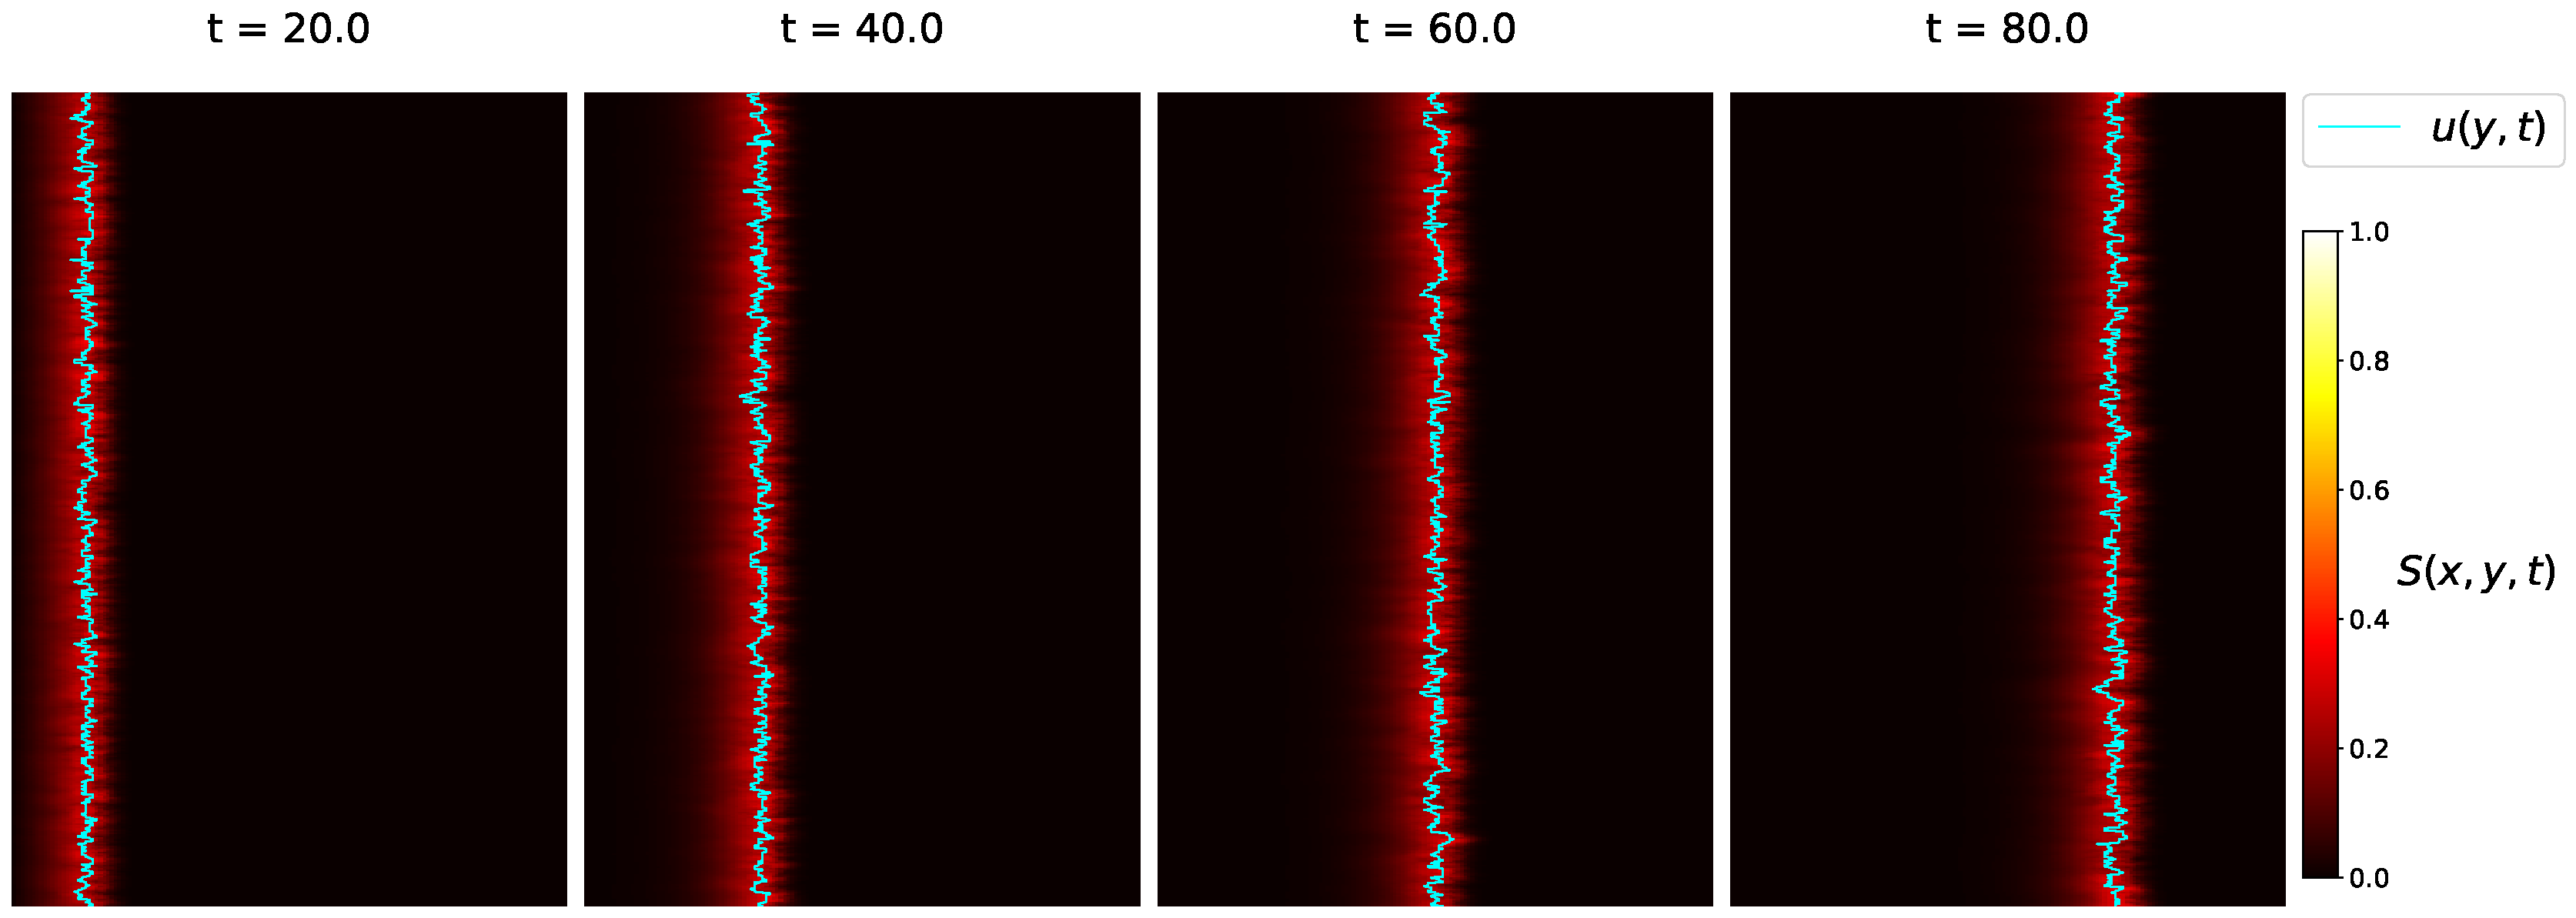
\includegraphics[width=\imsizeL]{hetal_case_tevol.pdf}
    \caption{Evolución del frente de infección/incendio para el problema heterogéneo dicotómico-aleatorio con $p=0.3$, $\gamma/\beta=0.2$ y $D_{I}=1$.}
    \label{fig:hom_case_tevol_hetero}
\end{figure}

\subsubsection*{Velocidad y amplitud del frente}

En la figura \ref{fig:u_cm(t)_hetal} se muestra la posición del centro de masa del frente de propagación $u_{cm}(t)$ en función del tiempo para
realizaciones de la simulación con $70$ valores distintos de $p\in(0,0.95)$. Puede observarse que para valores de $p$ grandes ($p\geq 0.9$) hay un cambio de comportamiento apreciable, 
las trayectorias comienzan a ser inestables y la velocidad media del frente se reduce drásticamente, ya que lleva más tiempo llegar al mismo lugar. Este cambio de 
comportamiento como consecuencia del valor de $p$ es de interés, ya que pareciera haber un valor crítico $p_c$
para el que el frente de infección reduce drásticamente su velocidad a un punto tal en que es difícil incluso identificar un frente. Este hecho también puede 
apreciarse en la figura \ref{fig:rugosidad} donde se muestra la rugosidad del campo de desplazamiento del frente (\ref{rugosidad}) en función de la posición del 
centro de masa. Para valores de $p\geq 0.9$ la rugosidad no deja de crecer mientras que para valores menores de $p$ 
la rugosidad se estabiliza alrededor de un valor dado. Adicionalmente, la rugosidad es un orden de magnitud mayor en los casos en que $p\geq 0.9$ comparada con las 
demás, esto también habla de una disipación del frente de onda al punto en que es irreconocible.

\begin{figure}[H]
    \centering
    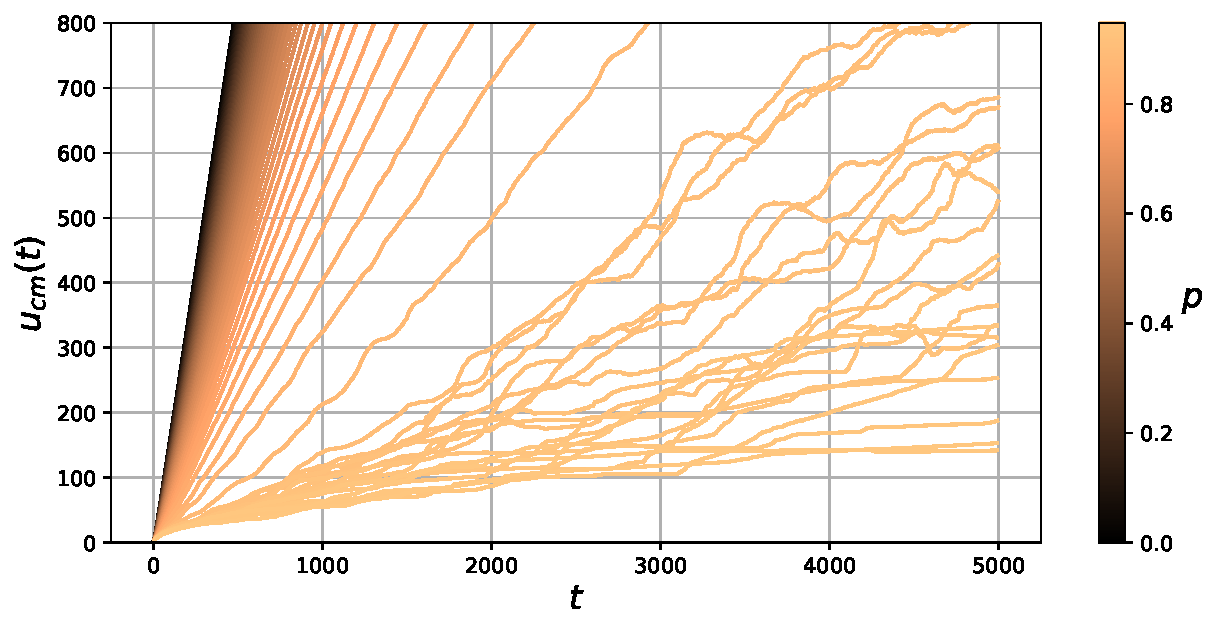
\includegraphics[width=\imsizeL]{u_cm(t)_hetal.pdf}
    \caption{Posición del centro de masa del frente de propagación en función del tiempo para distintos valores de $p$,con $\gamma/\beta=0.2$ y $D_{I}=1$.}
    \label{fig:u_cm(t)_hetal}
\end{figure}
\begin{figure}[H]
    \centering
    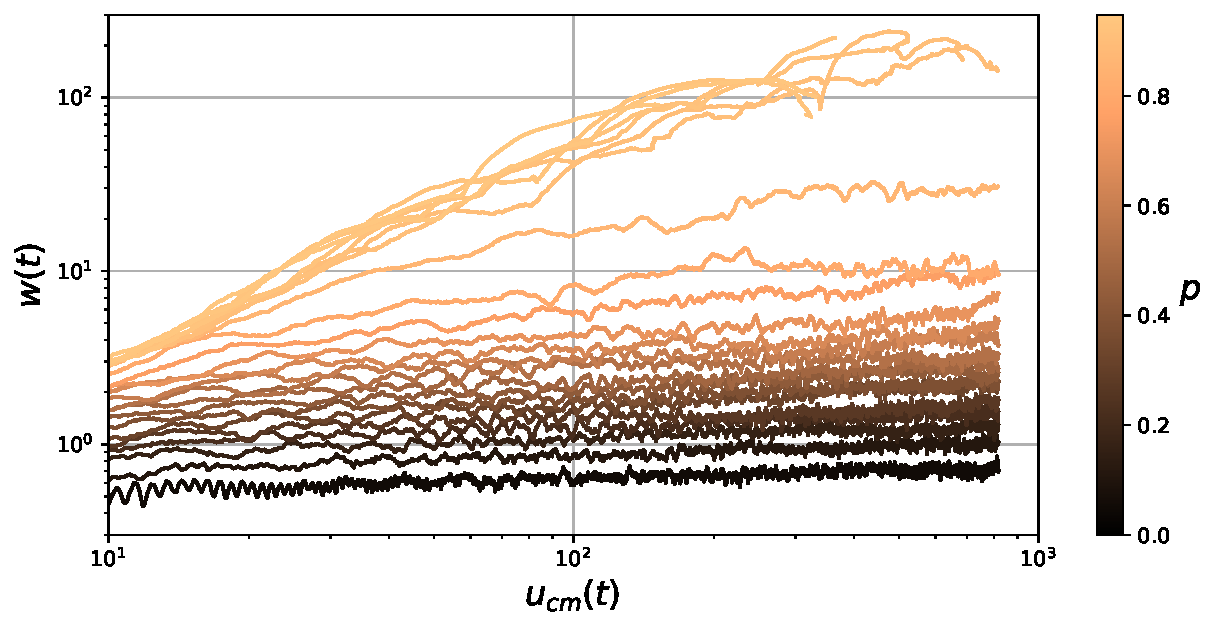
\includegraphics[width=\imsizeL]{rugosidad.pdf}
    \caption{Rugosidad $w(t)$ en función de la posición del centro de masa para distintos valores de $p$,con $\gamma/\beta=0.2$ y $D_{I}=1$.}
    \label{fig:rugosidad}
\end{figure}

Para poder determinar el valor crítico $p_c$ en el que se produce este cambio de comportamiento, calculamos a partir de los resultados de la figura \ref{fig:u_cm(t)_hetal}
la velocidad de propagación $c$ para los distintos valores de $p$ usando ajustes lineales. Los resultados obtenidos se muestran en la figura \ref{fig:velocidad_p}.
Se observa este procedimiento para dos sistemas distintos con $\gamma/\beta=0.2$ y $0.4$ y $D_{I}=1$. Además, se muestran estos mismos resultados para los mismos 
sistemas simulados sobre un medio homogéneo (H) con una tasa de transmisión igual a la media de sus pares heterogéneos dicotómicos-aleatorios (DA). Vemos que en ambos casos la velocidad 
del frente es menor sobre el medio homogéneo que sobre el heterogéneo y la diferencia entre ambas velocidades incrementa con $p$. Este tipo de resultado no es 
trivial y como es propio de los sistemas complejos no siempre es posible desarrollar una intuición apropiada para describir fenómenos emergentes de este tipo.
Es decir, con la misma tasa de transmisión media, una distribución homogénea sobre el espacio da lugar a un frente de propagación de menor velocidad 
que una distribución heterogénea dicotómica y aleatoria. 

Se realizó un ajuste con la regla de potencia $c\propto(1-p/p_c)^{\alpha_c}$ para las realizaciones sobre el medio homogéneo en todo el rango de $p$. De lo cual se 
obtuvo $p_c \approx 0.8$ y $0.6$ para $\gamma/\beta=0.2$ y $0.4$ respectivamente con exponente crítico $\alpha_c \approx 0.5$ para ambos. Esto concuerda con lo que 
resulta de reemplazar $\beta$ por $(1-p)\beta$ en la ecuación para la velocidad sobre medios homogéneos determinada en \ref{ondas}, es decir,

\[c(p) = 2\sqrt{D_I((1-p)\beta S_0-\gamma)} = c_0(1-p/p_c)^{\alpha_c},\]
con $p_c=1-\gamma/(\beta S_0)$ y $\alpha_c=0.5$. 


\begin{figure}[h]
    \centering
    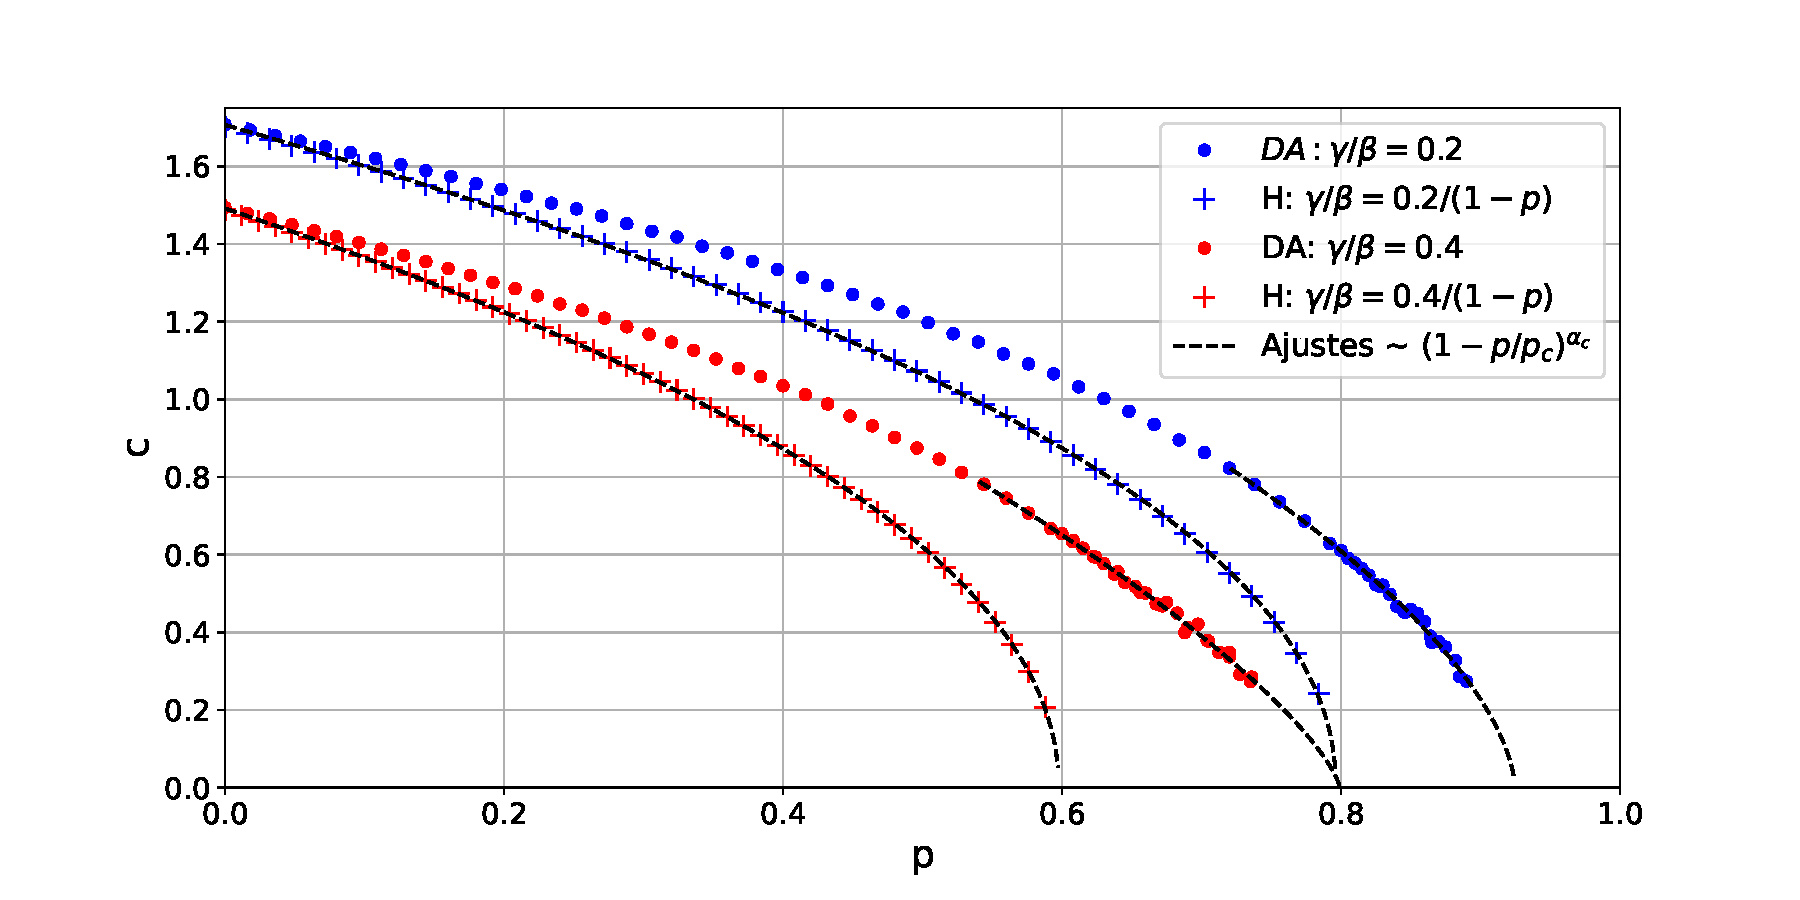
\includegraphics[width=\imsizeL]{velocidad_p.pdf}
    \caption{Velocidad $c$ del frente de propagación en función de $p$ con $\gamma/\beta=0.2$ y $0.4$ y $D_{I}=1$. Se muestran los 
    ajustes con la regla de potencia $c\propto(1-p/p_c)^{\alpha_c}$ sobre la región crítica.}
    \label{fig:velocidad_p}
\end{figure}

Por otro lado, para los medios DA se realizó un ajuste similar sobre las regiones críticas  de $p$. Todos los resultados asociados a los parámetros críticos de 
la velocidad determinados para cada caso se muestran en la tabla \ref{tab:param_criticos}. 

\begin{table}[]
    \centering
    \caption{Parámetros críticos $p_c$ y $\alpha_c$ de los medios H y DA con diferentes $\gamma/\beta$.}
    \label{tab:param_criticos}
    \begin{tabular}{@{}cccc@{}}
    \toprule
    Medio & $\gamma/\beta$ & $p_c$         & $\alpha_c$    \\ \midrule
    DA    & 0.2            & $0.92\pm0.04$ & $0.61\pm0.05$ \\
    H     & 0.2            & $0.80\pm0.01$ & $0.47\pm0.04$ \\
    DA    & 0.4            & $0.80\pm0.04$ & $0.73\pm0.05$ \\
    H     & 0.4            & $0.60\pm0.01$ & $0.48\pm0.04$ \\ \bottomrule
    \end{tabular}
\end{table}

De estos resultados queda claro otra diferencia importante entre los casos H y DA, y es que el valor crítico de $p$ para el cual se extingue el frente 
de propagación es apreciablemente mayor en los casos heterogéneos, hasta un $30\%$ mayor en el caso de $\gamma/\beta=0.4$. 

Es posible realizar un procedimiento similar determinando la amplitud media del frente de infección $I_{max}$ (\ref{Imax}) para distintas realizaciones variando el 
valor de $p$. En la figura \ref{fig:amplitud_p} se muestran los resultados obtenidos. En este caso vemos que sale desfavorecido el medio homogéneo ya que 
la amplitud media $I_{max}$ del frente de infección resulta ser mayor que en el medio aleatorio.
Se realizó asimismo un ajuste con la regla $(1-p/p_c)^{\alpha_I}$ para los casos heterogéneos sobre las regiones críticas, en la tabla \ref{tab:param_criticos_I} 
se muestran los resultados obtenidos.

\begin{table}[h]
    \centering
    \caption{Parámetros críticos $p_c$ y $\alpha_I$ del medio DA con diferentes $\gamma/\beta$.}
    \label{tab:param_criticos_I}
    \begin{tabular}{@{}cccc@{}}
    \toprule
    Medio & $\gamma/\beta$ & $p_c$         & $\alpha_I$    \\ \midrule
    DA    & 0.2            & $0.90\pm 0.04$ & $1.93 \pm 0.05$ \\
    DA    & 0.4            & $0.75\pm 0.04$ & $2.12 \pm 0.05$ \\ \bottomrule
    \end{tabular}
\end{table}

Puede verse que dentro del error, los resultados obtenidos para $p_c$ concuerdan con los obtenidos del ajuste para la velocidad. Por otro lado, es posible observar que 
tanto para el caso de la amplitud media como de la velocidad los exponentes críticos difieren del dado en los casos homogéneos y también difieren entre sí.


 \begin{figure}[H]
    \centering
    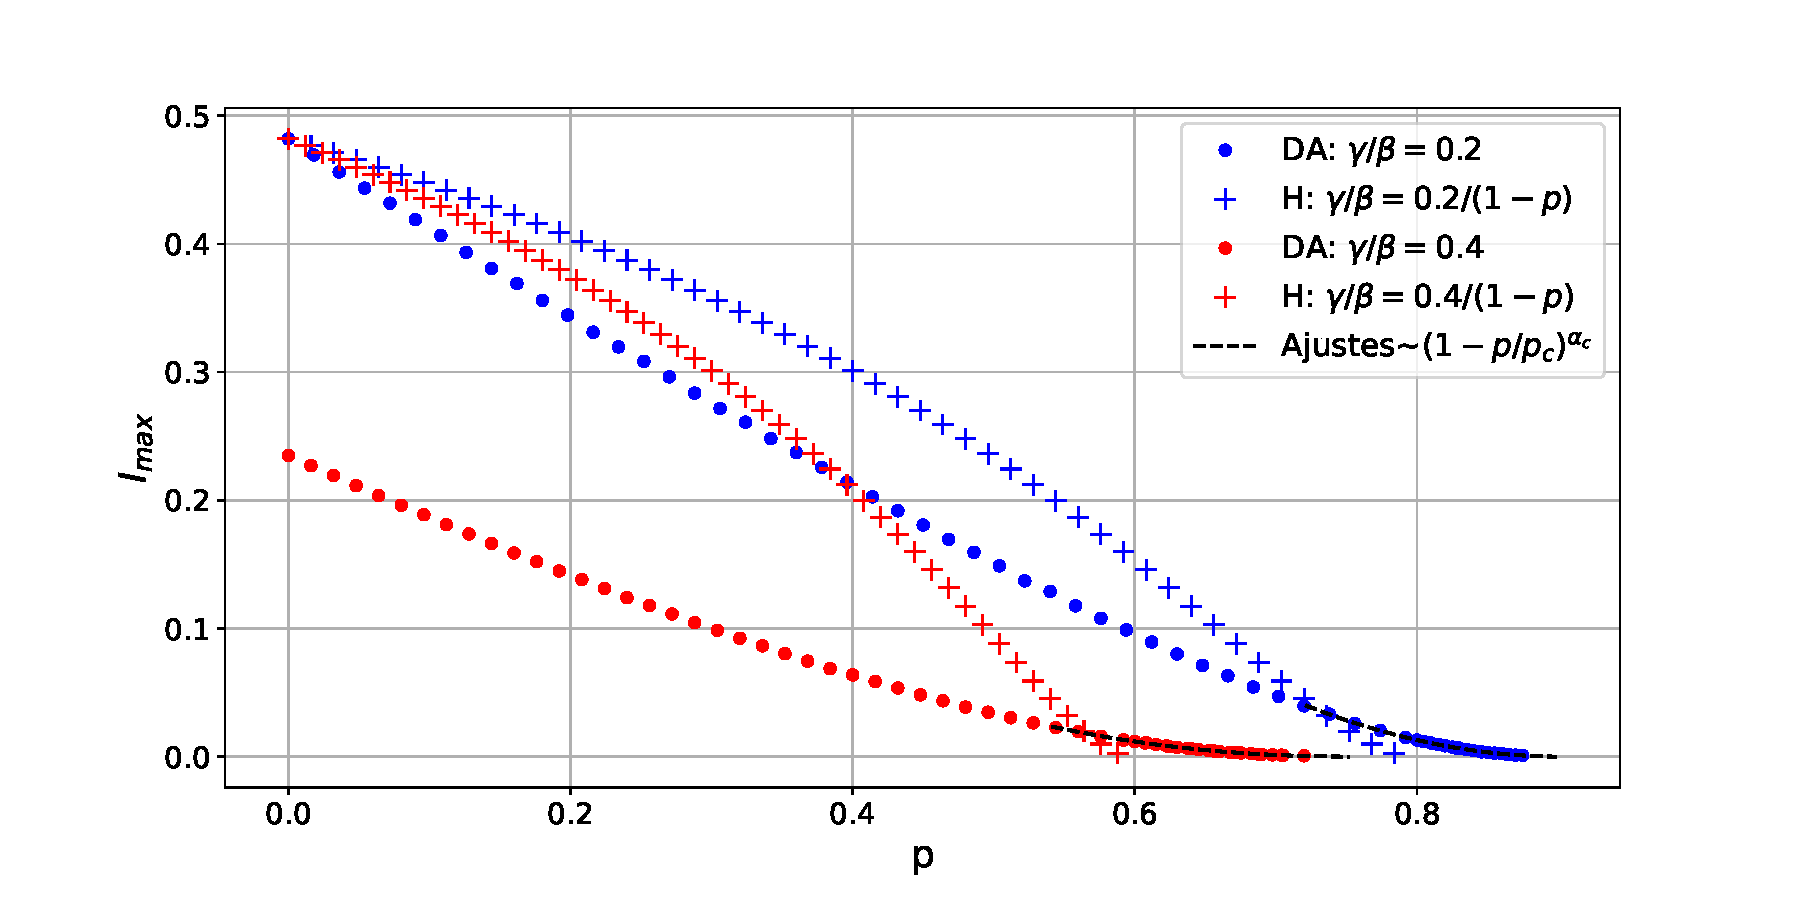
\includegraphics[width=\imsizeL]{amplitud_p.pdf}
    \caption{Amplitud media $I_{max}$ del frente de propagación en función de $p$ con $\gamma/\beta=0.2$ y $0.4$ y $D_{I}=1$. Se muestran los 
    ajustes con la regla de potencia $I_{max}\propto(1-p/p_c)^{\alpha_I}$ sobre la región crítica.}
    \label{fig:amplitud_p}
 \end{figure}
 
 Para ver más resultados asociados a esta heterogeneidad se puede consultar el artículo \cite{kolton}. Allí se presentan resultados adicionales acerca del factor de 
 estructura del frente $S(q)$ (\ref{factor}) y del perfil del frente $f_I(x)$. Se encuentra una estructura auto-afín del frente sobre la región crítica, con una ley 
 del tipo $S(q)\propto 1/q^{1+2\zeta}$.

 En resumen, los resultados obtenidos aquí pueden describirse cualitativamente de la siguiente manera: 
 \begin{itemize}
     \item Si el valor medio de la tasa de transmisión $\overline{\beta_{\vb r}}$ es el mismo, la velocidad del frente de infección/incendio es \textit{mayor} sobre el medio 
     dicotómico-aleatorio que sobre el homogéneo.
     \item Si el valor medio de la tasa de transmisión $\overline{\beta_{\vb r}}$ es el mismo, la amplitud media del frente de infección/incendio $I_{max}$ es 
     \textit{mayor} sobre el medio homogéneo que sobre el dicotómico-aleatorio en tanto $p<p_c$, con $p_c$ del medio homogéneo.
     \item El valor crítico $p_c$ para el cual se extingue el frente de infección/incendio es \textit{mayor} sobre el medio dicotómico-aleatorio que sobre el homogéneo.
     \item Los exponentes críticos de la velocidad $\alpha_c$ para el medio homogéneo \textit{coinciden} con el estimado por $c_0$ en la aproximación analítica de la solución de onda.
     \item Los exponentes críticos de la velocidad $\alpha_c$ para el medio dicotómico-aleatorio son \textit{mayores} que para el medio homogéneo y parecen 
     \textit{variar} con $\gamma/\beta$.
 \end{itemize}

 
\section{Medios correlacionados}

En esta sección estudiamos las heterogeneidades con correlación introducidas en la sección \ref{S:Modelo SIR espacial het}, estas son las denominadas 
<<suavizada>> (S) y <<dicotómica-correlacionada>> (DC). 

En las figuras \ref{fig:suavizada} y \ref{fig:suavizada-dicotómica} se muestra la evolución temporal del sistema para 
$p=0.3$ y con un paso de suavizado para cada caso, es decir, con $\beta_{\vb r}^{(1)}$ y $\tilde{\beta}_{\vb r}^{(1)}$ respectivamente. Puede verse que DC presenta un 
campo de desplazamiento más rugoso que S y que la velocidad del frente en S es mayor que en DC. Sin embargo, aquí nuevamente resulta que la comparación es injusta 
ya que, aunque ambas simulaciones están hechas con el mismo valor de $p$, tienen distinta tasa de transmisión media. Como se vió en la sección 
\ref{S:Modelo SIR espacial het}, el valor medio sobre S es $\overline{\beta_{\vb r}^{(n)}}=(1-p)\beta$ mientras que sobre DC 
el valor medio de la tasa de transmisión cambia. Por ello utilizaremos de ahora en más como parámetro de referencia el valor medio de la tasa de transmisión y no $p$.


\begin{figure}[h]
    \centering
    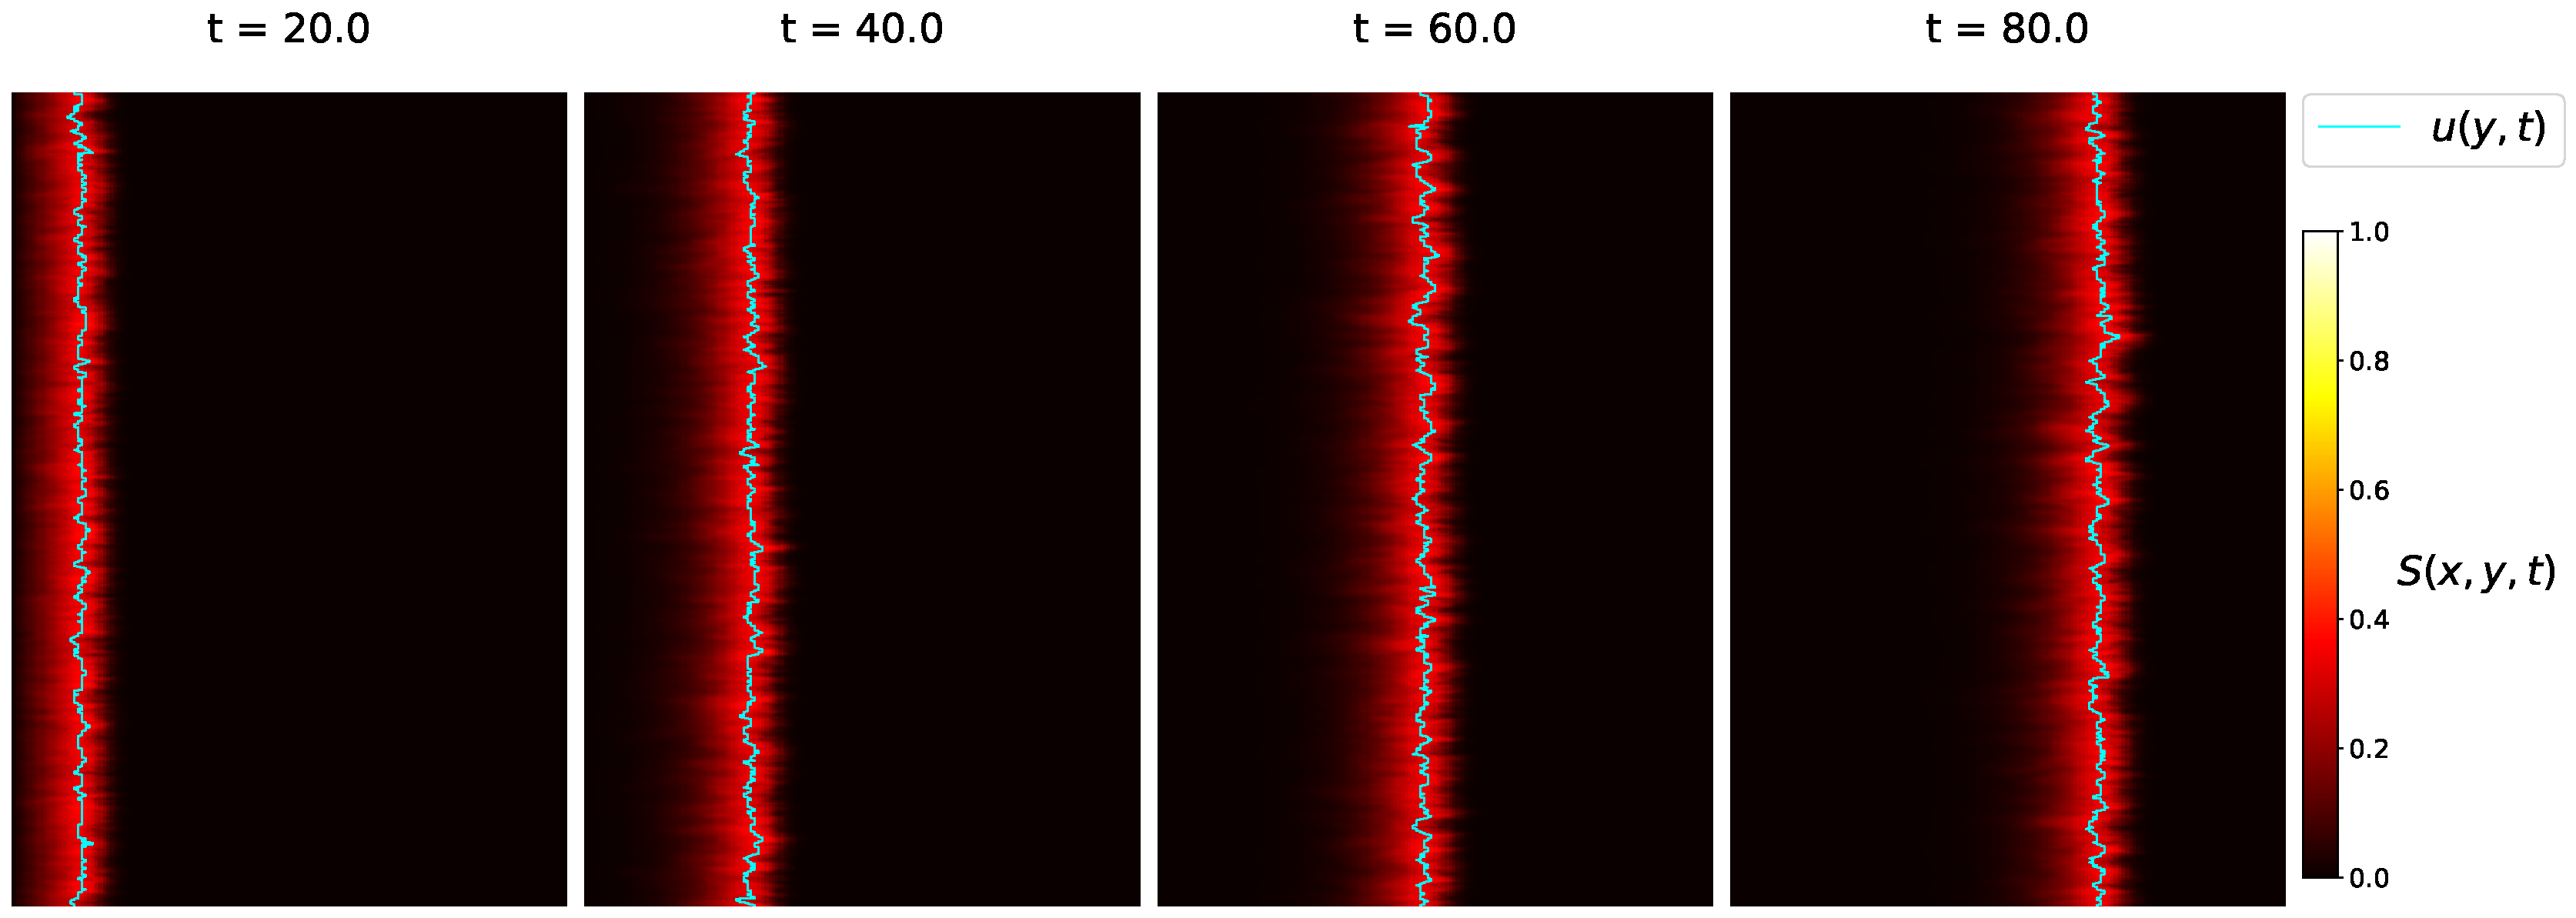
\includegraphics[width=\imsizeL]{suavizada_tevol.pdf}
    \caption{Evolución temporal del sistema para $p=0.3$ con un paso de S.}
    \label{fig:suavizada}
\end{figure}

\begin{figure}[h]
    \centering
    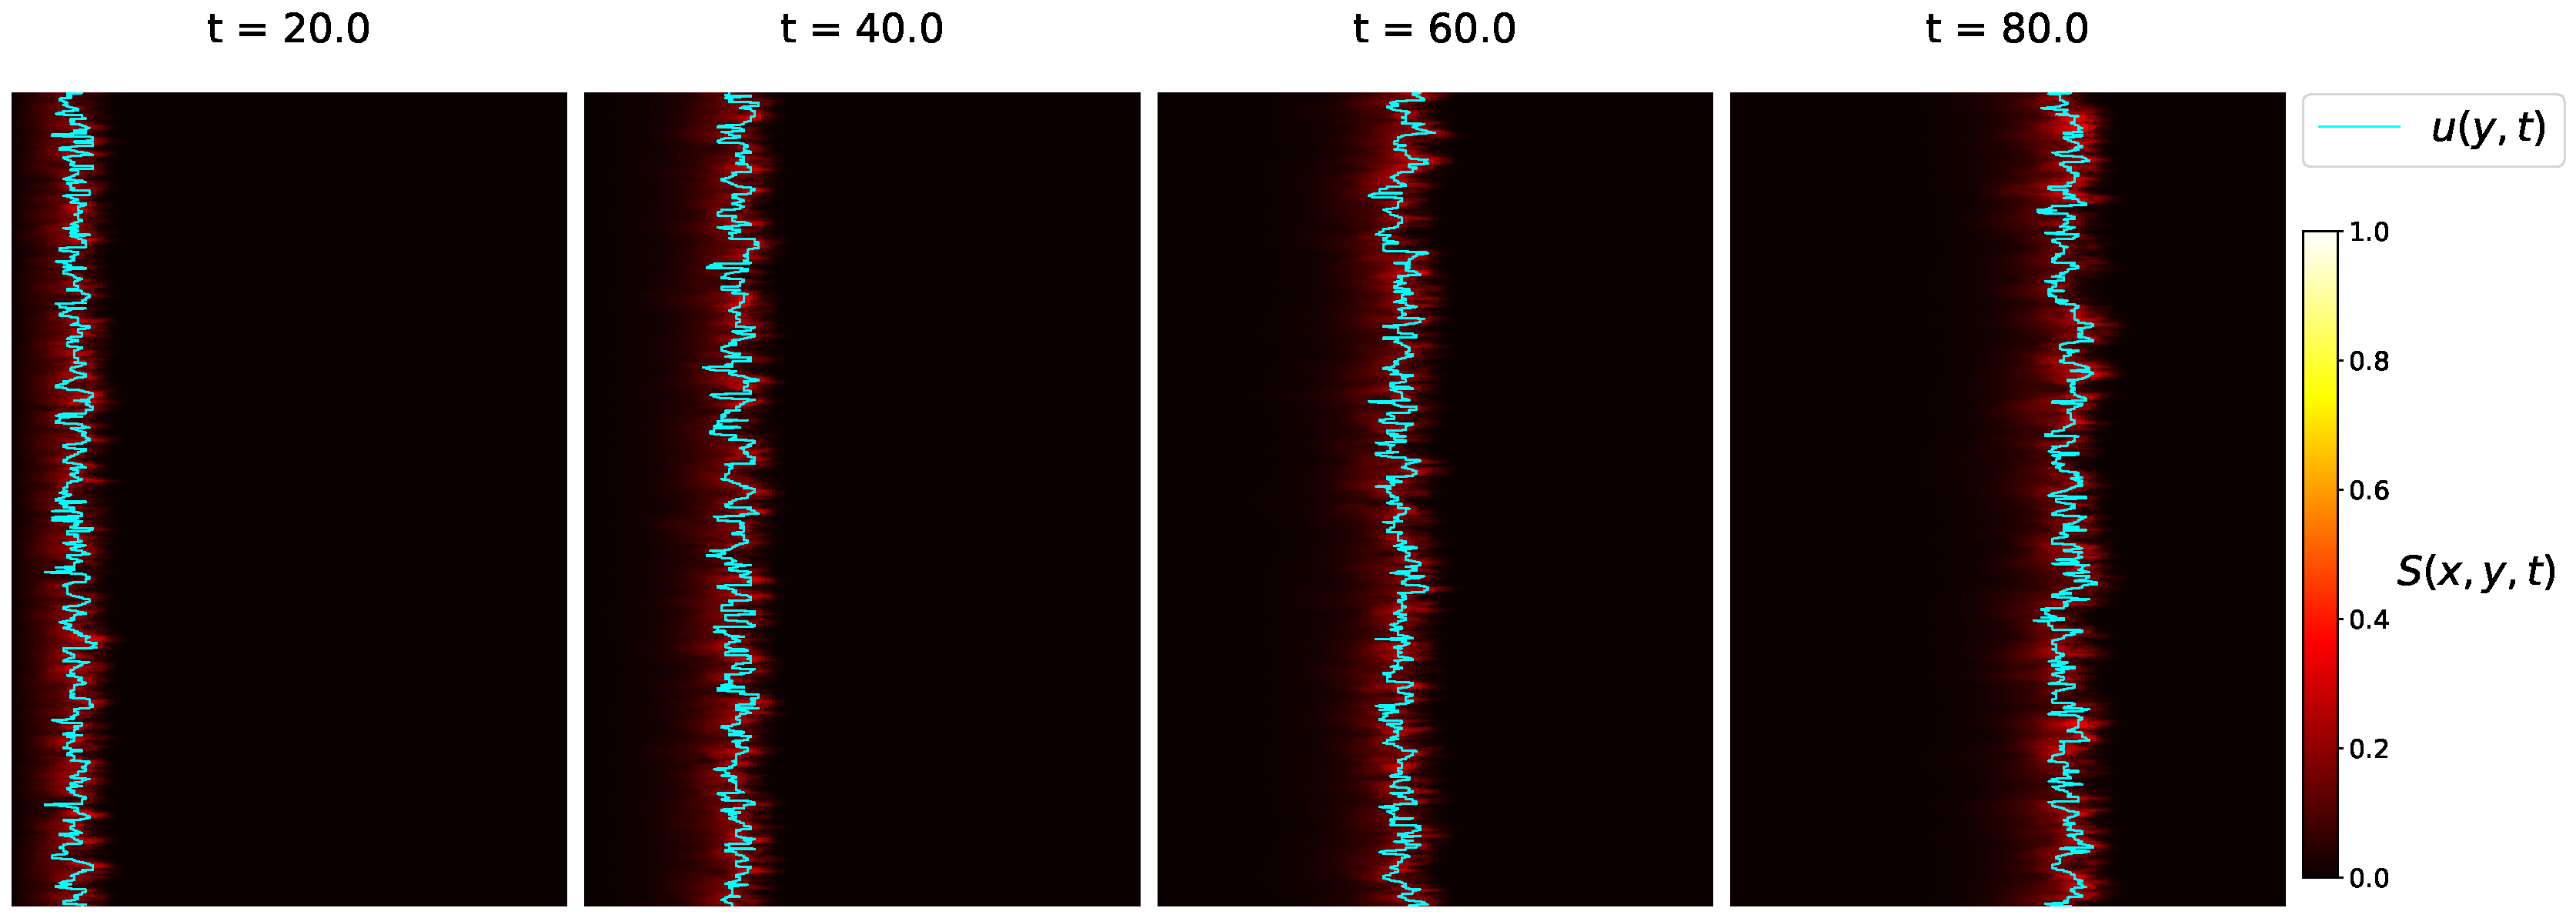
\includegraphics[width=\imsizeL]{suavizada_dic_tevol.pdf}
    \caption{Evolución temporal del sistema para $p=0.3$ con un paso de DC.}
    \label{fig:suavizada-dicotómica}
\end{figure}

\subsection{Velocidad y amplitud del frente}

En las figuras \ref{fig:ucm_s} y \ref{fig:ucm_sd} se muestra la posición del centro de masa del frente de realizaciones con distinta tasa 
de transmisión media, para S y DC respectivamente. Se utilizó $\gamma=0.2$, $\beta=1$ y $D_I=1$. 

Se puede apreciar, en ambos casos, que mientras mayor es la tasa 
de transmisión media, mayor es la velocidad del frente de infección/incendio, esto es algo de esperar. Sin embargo, algo que llama la atención 
es que el frente de infección parece sostener una velocidad mayor sobre DC que sobre S a medida que disminuye $\overline{\beta_{\vb r}}$.

\begin{figure}[h]
    \centering
    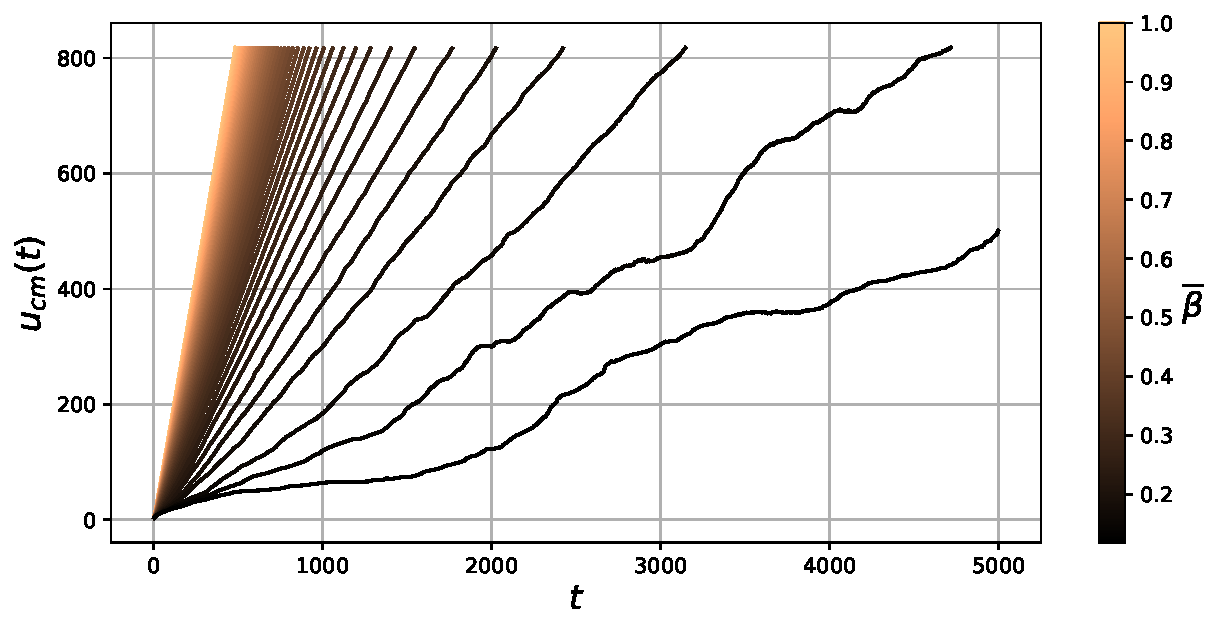
\includegraphics[width=\imsizeL]{ucm_s.pdf}
    \caption{Posición del centro de masa del frente en función del tiempo sobre el medio S.}
    \label{fig:ucm_s}
\end{figure}
\begin{figure}[h]
    \centering
    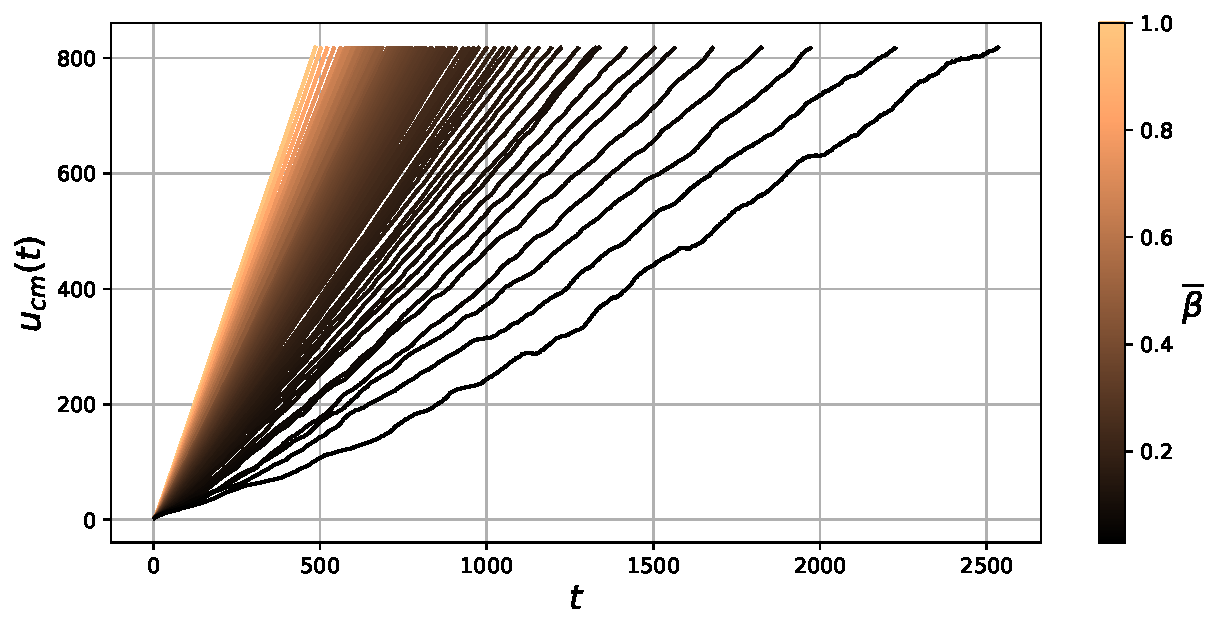
\includegraphics[width=\imsizeL]{ucm_sd.pdf}
    \caption{Posición del centro de masa del frente en función del tiempo sobre el medio DC.}
    \label{fig:ucm_sd}
\end{figure}

Lo mencionado anteriormente queda claro al observar la figura \ref{fig:c_all}, donde se muestra la velocidad en función de $\overline{\beta_{\vb r}}$ sobre los medios
S y DC con un paso de suavizado. Adicionalmente, se muestran las curvas equivalentes para los medios homogéneo (H) y dicotómico-aleatorio (DA), vistos en \ref{S:aleatorios}. 
Vemos que la curva asociada a S queda entre las curvas de los medios H y DA. Esto es razonable ya que S se genera a partir de DA y como vimos 
en la sección \ref{S:Modelo SIR espacial het}, el medio S tiende a uno homogéneo con $\overline{\beta_{\vb r}}=(1-p)\beta$ cuando incrementamos los pasos de suavizado.
Es de esperar entonces que curvas similares sobre S pero con más pasos de suavizado vayan asemejándose cada vez más a la versión homogénea.

\begin{figure}[h]
    \centering
    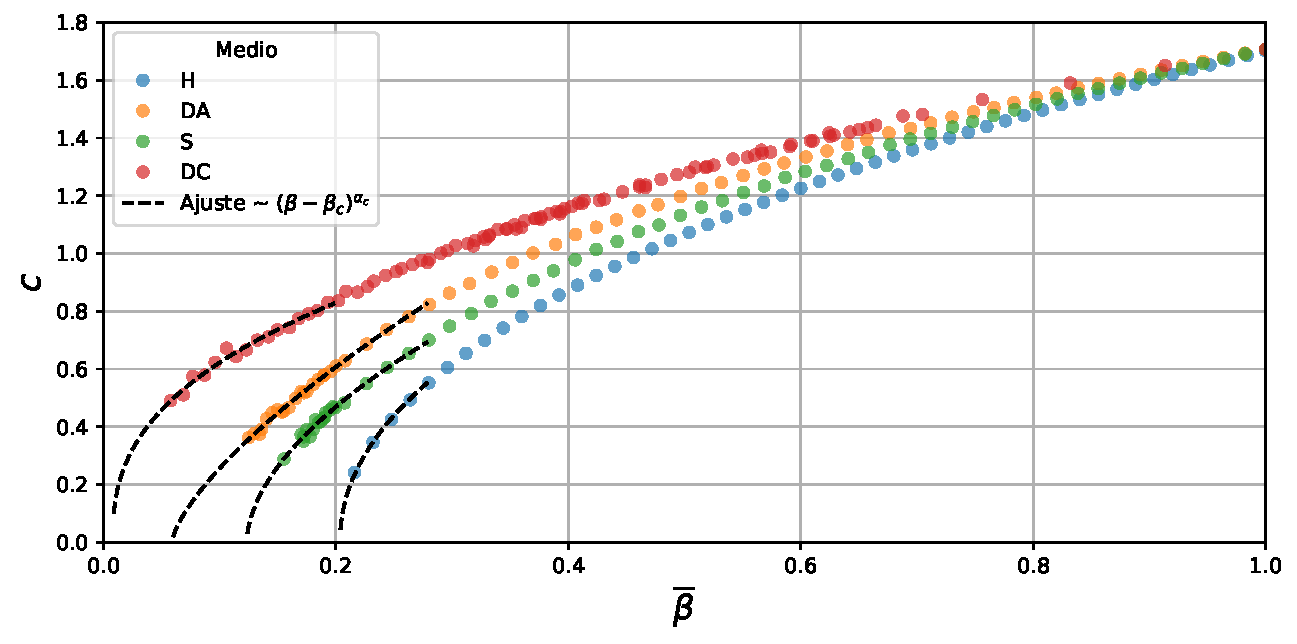
\includegraphics[width=\imsizeL]{c_all.pdf}
    \caption{Velocidad del frente de infección en función del valor medio de la tasa de transmisión $\overline{\beta_{\vb r}}$ sobre los medios S, DC, DA y 
    H. Se muestran los ajustes con la regla de potencia $c\propto(\beta-\beta_c)^{\alpha_c}$ sobre la región crítica.}
    \label{fig:c_all}
\end{figure}

Por otro lado, la curva asociada a DC queda alejada de las demás, se observa que la velocidad del frente es apreciablemente más grande que en los 
demás casos cuando la tasa de transmisión media es chica, $\overline{\beta_{\vb r}}<0.2$. Ahora bien, este resultado por sí mismo es por lo menos curioso, es decir,
\textbf{un ligero cambio en la estructura del medio sin afectar la tasa de transmisión media produce un cambio notable en la velocidad del frente}. Fundamentalmente, 
comparando el resultado de DC con el de DA, a pesar de que ambos medios tengan un carácter dicotómico, la correlación espacial introducida en DC genera 
un cambio notable sobre la velocidad.

Para entender mejor qué es lo que produce este cambio de velocidad entre DA y DC es interesante observar con mayor detenimiento la estructura de estos medios. En las 
figuras \ref{beta_al_zoom} y \ref{beta_dic_zoom} se muestra la distribución de la tasa de transmisión $\beta_{\vb r}$ sobre el espacio de los medios DA y DC respectivamente. 
Ambos casos tienen la misma tasa de transmisión media. Observando la distribución espacial de cada uno de ellos 
a gran escala, sobre el espacio de $1024\times1024$, no es sencillo señalar ninguna diferencia. Sin embargo, al observar la distribución sobre una región acotada de 
$100\times100$ se puede ver que son estructuralmente distintos en esta escala. La distribución de CD con $n=1$ alcanza a formar un patrón  
distinguible, se forman regiones agrupadas con tasa de transmisión no nula $\beta$, mientras que en DA, por supuesto, se observa el carácter aleatorio. Este es un 
fenómeno notable, la velocidad de propagación es mayor si la distribución de la tasa de transmisión forma estructuras como las que se ven en la figura 
\ref{beta_dic_zoom} en lugar de estar distribuída aleatoriamente, por más que la tasa de transmisión media sea la misma.

\begin{figure}[H]
    \centering
    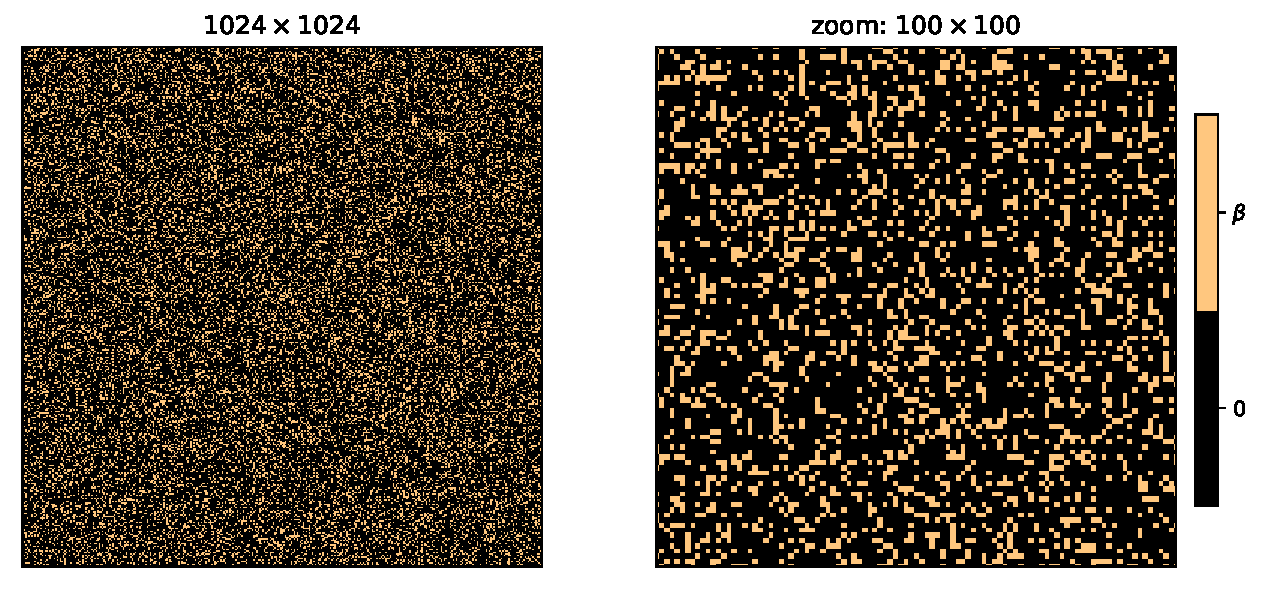
\includegraphics[width=\imsize]{beta_al_zoom.pdf}
    \caption{Distribución de la tasa de transmisión $\beta_{\vb r}$ del medio DA. A izquierda se muestra la distribución sobre 
    todo el espacio de $1024\times1024$ y a la derecha un acercamiento a una región de $100\times100$.}
    \label{beta_al_zoom}
\end{figure}
\begin{figure}[H]
    \centering
    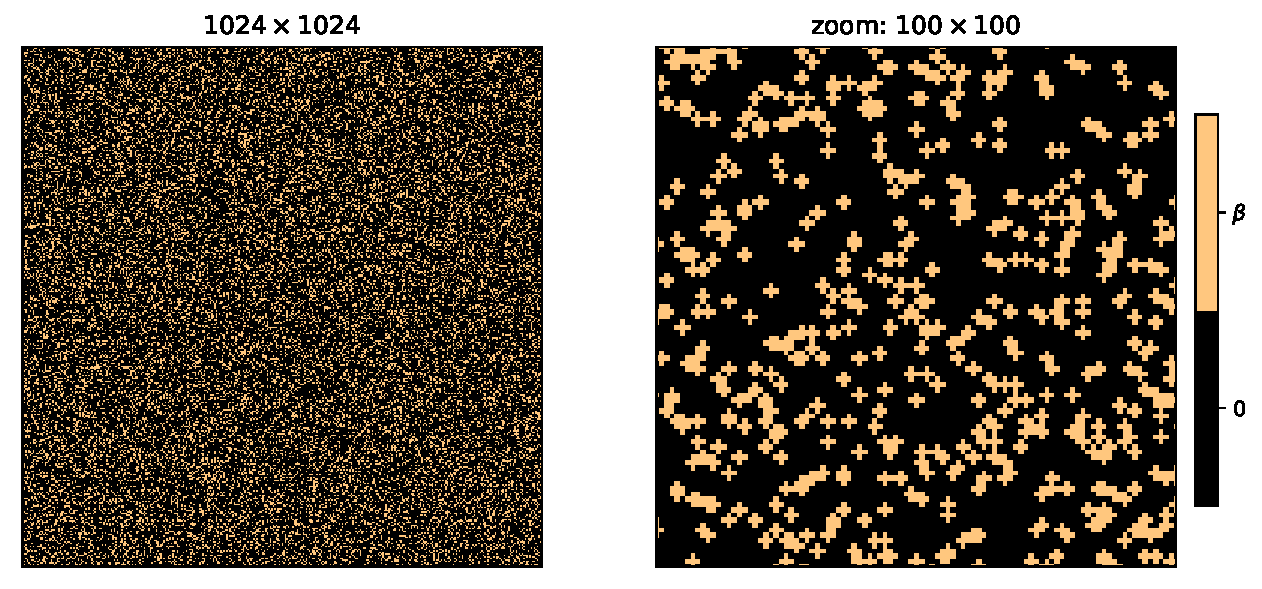
\includegraphics[width=\imsize]{beta_dic_zoom.pdf}
    \caption{Distribución de la tasa de transmisión $\beta_{\vb r}$ del medio DC. A izquierda se muestra la distribución sobre 
    todo el espacio de $1024\times1024$ y a la derecha un acercamiento a una región de $100\times100$.}
    \label{beta_dic_zoom}
\end{figure}

Se realizaron ajustes con la regla de potencia $c\propto(\beta-\beta_c)^{\alpha_c}$ sobre la región crítica para los medios DC, DA, S y H. De ello se determinó la tasa de 
transmisión crítica y el exponente crítico para cada uno de ellos. En la tabla \ref{tab:pc} se muestran los resultados obtenidos.

\begin{table}[h]
    \centering
    \caption{Parámetros críticos $\beta_c$ y $\alpha_c$ de los medios DC, DA ,S y H.}
    \label{tab:pc}
    \begin{tabular}{@{}cccc@{}}
    \toprule
    Medio & $\beta_c$     & $\alpha_c$    \\ \midrule
    H     & $0.20\pm0.01$ & $0.48\pm0.03$ \\
    DA    & $0.06\pm0.02$ & $0.70\pm0.05$ \\
    DC    & $0.01\pm0.01$ & $0.39\pm0.05$ \\
    S     & $0.12\pm0.02$ & $0.55\pm0.05$ \\ \bottomrule
    \end{tabular}
\end{table}

Puede verse que los resultados sobre los medios $H$ y $DA$ coinciden con los valores críticos $p_c$ obtenidos en la sección anterior (Tabla \ref{tab:param_criticos}).
Esto era de esperar dado que sobre estos medios, la tasa de transmisión media y el valor de $p$ están relacionados por $\overline{\beta_{\vb r}}=(1-p)\beta$, de modo que 
$\beta_c=(1-p_c)\beta$. De estos resultados también queda claro otro fenómeno notable al que da lugar la estructura del medio DC, y es que sobre este la tasa 
de transmisión crítica es \textit{menor} comparada con las demás. Es decir, basta con una tasa de transmisión extremadamente chica, comparada con los demás medios,
para que tenga lugar un frente de propagación.

Otro aspecto de inteŕes es observar el efecto que tienen los distintos medios sobre la amplitud media del frente de infección/incendio . En la figura \ref{fig:I_all} se 
observa la amplitud media del frente como función de la tasa de transmisión media $\overline{\beta_{\vb r}}$ para los medios S, DC, DA y H. En esta ocasión vemos que el
medio homogéneo es el que sostiene la mayor amplitud del frente cuando $\overline{\beta_{\vb r}}>0.35$. Vemos aquí nuevamente que la curva de S queda entre las dadas 
por H y DA. Por otro lado, el medio DC, en consistencia con lo observado para la velocidad, otorga la mayor amplitud del frente para valores bajos de la tasa de
transmisión media $\overline{\beta_{\vb r}}<0.35$. Es decir, el medio DC favorece nuevamente, en este aspecto y sobre este régimen, a la propagación del frente.

\begin{figure}[h]
    \centering
    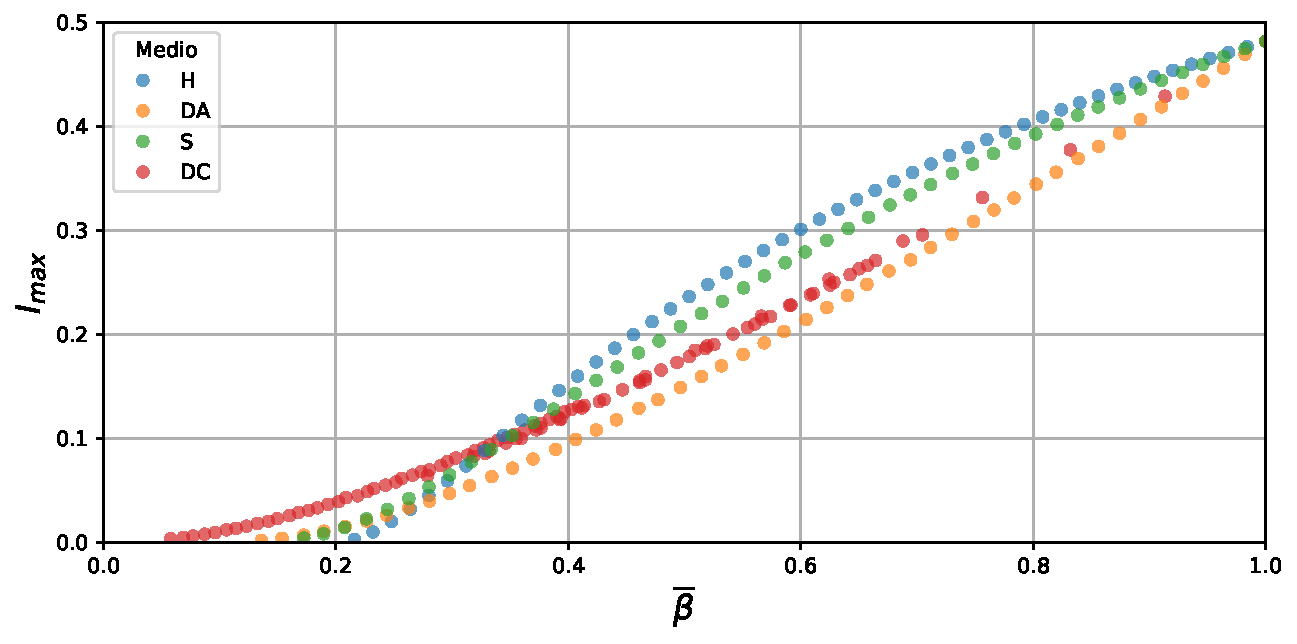
\includegraphics[width=\imsizeL]{I_all.pdf}
    \caption{Amplitud media del frente de infección/incendio $I_{max}$ en función de la tasa de transmisión media $\overline{\beta_{\vb r}}$ para los medios S, DA, 
    DC y H.}
    \label{fig:I_all}
\end{figure}

\subsection{Rugosidad y factor de estructura}

Ahora se propone investigar las propiedades geométricas del frente en función de $\overline{\beta_{\vb r}}$ cerca de los valores críticos $\beta_c$ obtenidos 
previamente para cada medio. En la figura \ref{width_beta} se muestra la rugosidad $\langle w(t)\rangle_t$ del frente de infección/incendio en función de la tasa de 
transmisión media para realizaciones sobre los medios S, DA y DC.

Para cada una de estas curvas se realizó un ajuste de tipo $\langle w(t)\rangle_t\propto(\beta-\beta_c)^{\alpha_c}$ sobre la región crítica. A partir de lo cual se 
obtuvieron los resultados que se muestran en la tabla \ref{tab:pc_I} para cada uno de los medios.

\begin{table}[h]
    \centering
    \caption{Parámetros críticos $\beta_c$ y $\alpha_w$ de los medios DC, DA y S.}
    \label{tab:pc_I}
    \begin{tabular}{@{}cccc@{}}
    \toprule
    Medio & $\beta_c$     & $\alpha_w$    \\ \midrule
    DA    & $0.07\pm0.02$ & $1.61\pm0.05$ \\
    DC    & $0.01\pm0.01$ & $0.96\pm0.05$ \\
    S     & $0.11\pm0.02$ & $1.48\pm0.05$ \\ \bottomrule
    \end{tabular}
\end{table}

Los valores críticos de $\beta_c$ concuerdan con los obtenidos previamente del estudio de la velocidad del frente, tal como corresponde (Tabla \ref{tab:pc}).

Por otro lado, si observamos el factor de estructura $S(q)$ (\ref{factor}) de los frentes cerca del valor crítico de la tasa de transmisión media, se observa que 
sobre el medio DA el frente presenta una estructura fractal auto-afín, $S(q)\sim 1/q^{1+2\zeta}$, con exponente de rugosidad $\zeta=0.3$ tal como puede verse de 
la figura \ref{fig:factor}. Sin embargo, para los medios S y DC no se observa nada similar, los valores de $\zeta$ son indistinguibles de cero.\newpage

\begin{figure}[h]
    \centering
    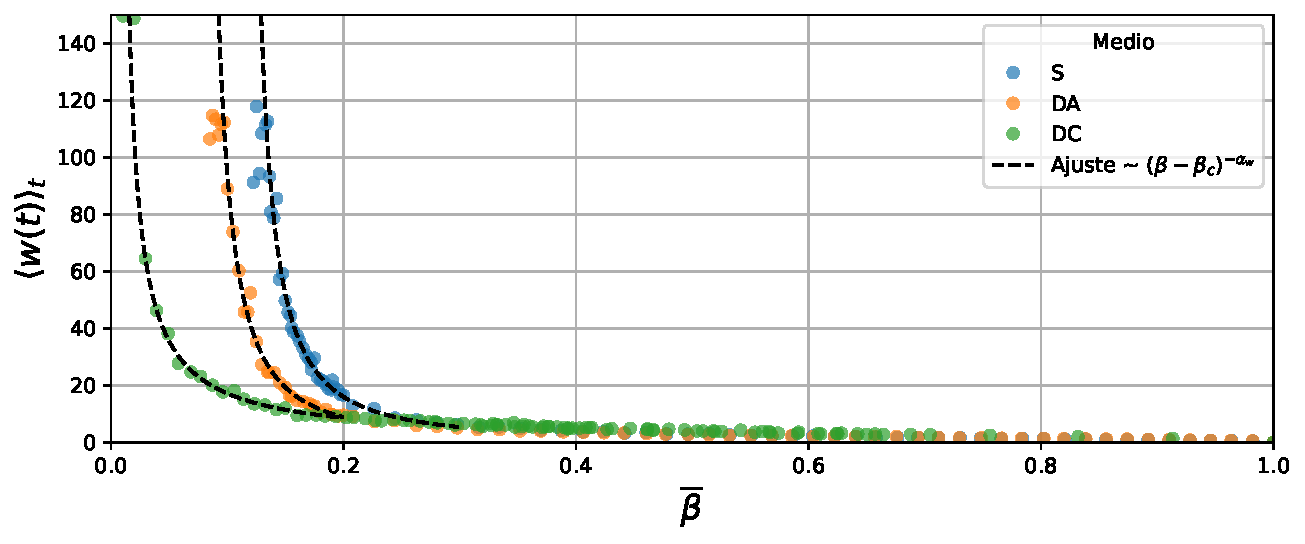
\includegraphics[width=\imsizeL]{width_beta.pdf}
    \caption{Rugosidad del frente de infección/incendio en función de la tasa 
    de transmisión media $\overline{\beta_{\vb r}}$ para los medios S, DA y DC.}
    \label{width_beta}
\end{figure}

\begin{figure}[h]
    \centering
    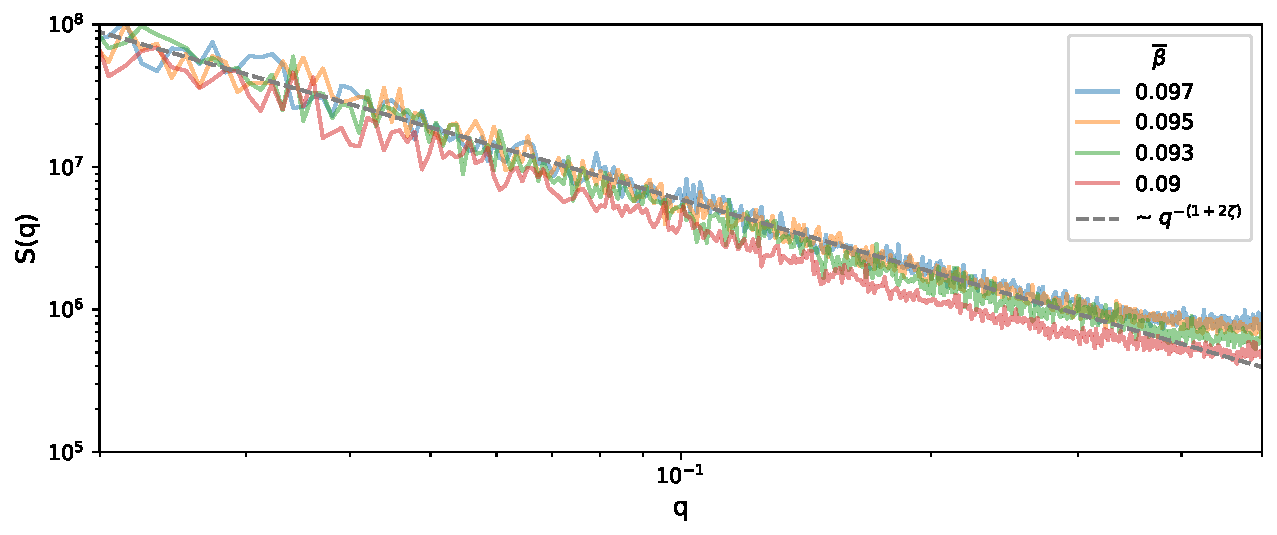
\includegraphics[width=\imsizeL]{factor.pdf}
    \caption{Factor de estructura $S(q)$ sobre el medio DA cerca de la tasa de transmisión cŕitica. Se muestra el ajuste $S(q)\sim 1/q^{1+2\zeta}$ con $\zeta\approx 0.3$.}
    \label{fig:factor}
\end{figure}

Resumiendo esta sección, se tienen los siguientes resultados:
\begin{itemize}
    \item Si la tasa de transmisión media es la misma, la velocidad del frente de infección/incendio es \textit{mayor} sobre el medio DC.
    \item Si la tasa de transmisión media es la misma y $\beta_{\vb r}>0.35$, la amplitud media del frente de infección/incendio es \textit{mayor} sobre el medio H.
    \item Si la tasa de transmisión media es la misma y $\beta_{\vb r}<0.35$, la amplitud media del frente de infección/incendio es \textit{mayor} sobre el medio DC.
    \item La tasa de transmisión crítica es la \textit{menor} sobre el medio DC y la \textit{mayor} sobre el medio H.
    \item Los exponentes críticos de la velocidad sobre los medios H, S, DA y DC parecen ser \textit{diferentes} entre sí, siendo el \textit{mayor} en el medio DA.
    \item El campo de desplazamiento del frente presenta una estructura auto-afín en el medio DA sobre el régimen crítico, $S(q)\propto q^{-(1+2\zeta)}$ con $\zeta=0.3$.
\end{itemize}

\section{Nocividad}

Un aspecto de gran importancia en lo que respecta a problemáticas tanto epidemiológicas como de incendios es la posibilidad de cuantificar los daños que
deja un brote de enfermedad infecciosa o un incendio. En particular, estaremos interesados en estimar el daño que queda tras el paso del frente de infección/incendio. 
Para ello utilizaremos como cuantificador de daños la fracción de susceptibles $S_1$ que queda tras el paso del frente de onda. Entendiendo que mientras menor sea esta 
fracción, mayor será el daño ocasionado por el frente.

Para ser más precisos al respecto, tomaremos 
\[S_1=\langle S(x,y,T)\rangle_{x,y}\]
con $0.2L<x<u_{cm}(T)-0.2L$, siendo $T$ el tiempo que dure la simulación correspondiente. Utilizando este criterio para todas las simulaciones, podremos comparar 
la nocividad de cada frente al modificar los parámetros que interesen. En particular, veremos cómo cambia esta magnitud $S_1$ con la tasa de transmisión media 
$\overline{\beta_{\vb r}}$.

En la figura \ref{fig:S_1} se muestran los resultados obtenidos de $S_1$ en función de $\overline{\beta_{\vb r}}$ sobre los medios H, S, DA y DC. Se puede 
observar que el frente de propagación más nocivo se da sobre el medio homogéneo, ya que da lugar a la menor fracción de susceptibles $S_1$ tras el paso del frente. Sin 
embargo, tal como ya hemos apreciado antes (Tabla \ref{tab:pc}), la tasa de transmisión crítica es menor que en los demás casos $\beta_c\approx0.2$.

\begin{figure}[h]
    \centering
    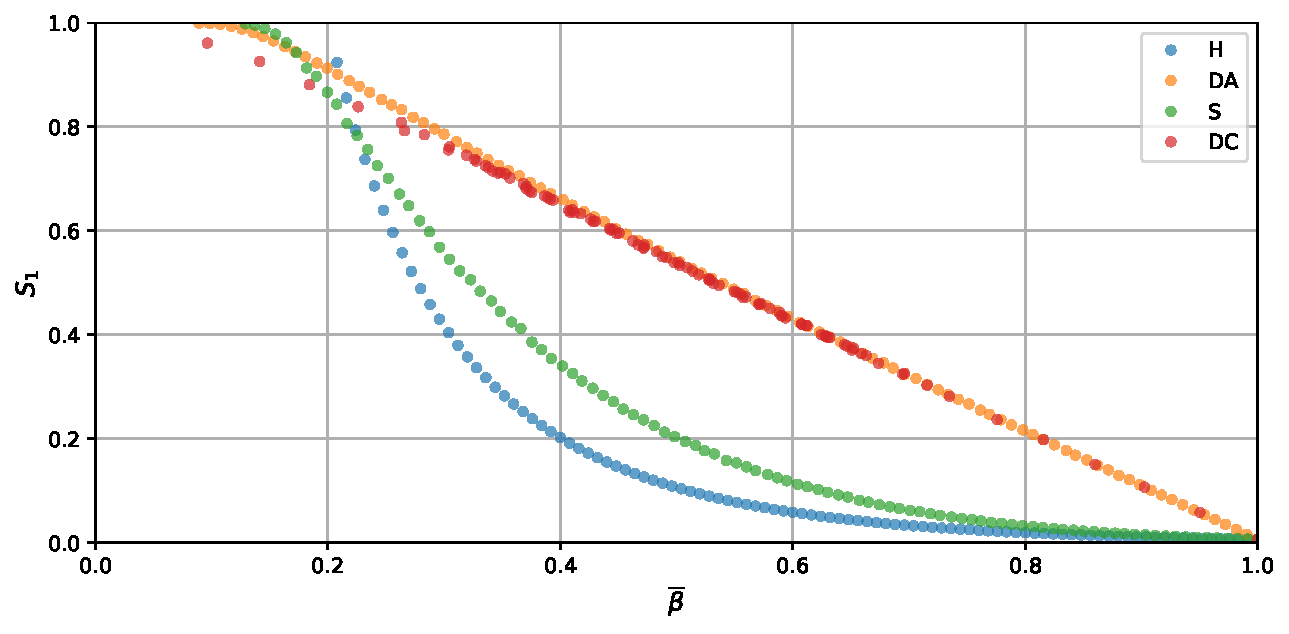
\includegraphics[width=\imsizeL]{S_1.pdf}
    \caption{Fracción de susceptibles $S_1$ en función de la tasa de transmisión media $\overline{\beta_{\vb r}}$ para los medios H, S, DA y DC.}
    \label{fig:S_1}
\end{figure}

El siguiente medio de nocividad elevada es S, mientras que los medios DC y DA presentan curvas similares de carácter lineal. Estos nuevos resultados dan una perspectiva 
nueva acerca de los medios. Por ejemplo, habíamos visto que la velocidad de propagación del frente es mayor sobre el medio DC que sobre los demás, lo cual es una 
característica indeseable en problemáticas tanto epidemiológicas como de incendios. Sin embargo, vemos ahora que a pesar de ello la nocividad del frente, tal como la
hemos caracterizado aquí, es menor sobre DC que sobre los demás medios, lo cual es deseable. A modo cualitativo es entendible que si el frente se desplaza a mayor 
velocidad tenga menos tiempo de ocasionar grandes daños. 

En resumen:

\begin{itemize}
    \item Si $\overline{\beta_{\vb r}}>0.2$, el frente de infección/incendio \textit{más nocivo} se da sobre el medio H.
    \item Si $\overline{\beta_{\vb r}}<0.2$, el frente de infección/incendio \textit{más nocivo} se da sobre el medio DC.
    \item Sobre los medios dicotómicos DC y DA, la \textit{nocividad} es directamente proporcional a la tasa de transmisión media, $S_1\propto\overline{\beta_{\vb r}}$.
\end{itemize}